\subsection{Terzo sprint}

\begin{minipage}{\textwidth}
  Di seguito è riportata la distribuzione delle ore per ciascun membro del team, accumulate in totali per persona e per ruolo:
  \begin{table}[H]
    \begin{tabularx}{\textwidth}{|c|*{6}{>{\centering}X|}c|}
      \hline
      \multicolumn{8}{|c|}{\textbf{Consuntivo orario}} \\
      \hline
      \textbf{Membro del team} & \textbf{Re} & \textbf{Am} & \textbf{An} & \textbf{Pt} & \textbf{Pr} & \textbf{Ve} & \textbf{Totale per persona} \\
      \hline
      Riccardo Cavalli & 1 & 2 & 0 & 6 & 2 & 0 & 11 \\
      \hline
      Raul Pianon & 0 & 0 & 0 & 0 & 8 & 0 & 8 \\
      \hline
      Martina Dall'Amico & 0 & 8 & 0 & 0 & 0 & 0 & 8 \\ 
      \hline
      Marco Cristo & 0 & 0 & 0 & 0 & 5 & 2 & 7 \\ 
      \hline
      Sebastiano Lewental & 0 & 0 & 0 & 3 & 2 & 3 & 8 \\ 
      \hline
      Mattia Zecchinato & 0 & 1 & 5 & 0 & 0 & 0 & 6 \\ 
      \hline
      Tommaso Stocco & 4 & 0 & 0 & 0 & 0 & 2 & 6 \\ 
      \hline
      \textbf{Totale ore per ruolo} & 5 & 11 & 5 & 9 & 17 & 7 & \textbf{54} \\
      \hline
    \end{tabularx}
    \caption{Sprint 3 - Consuntivo orario}
  \end{table}
  \end{minipage}
  
  \begin{figure}[H]
    \centering
    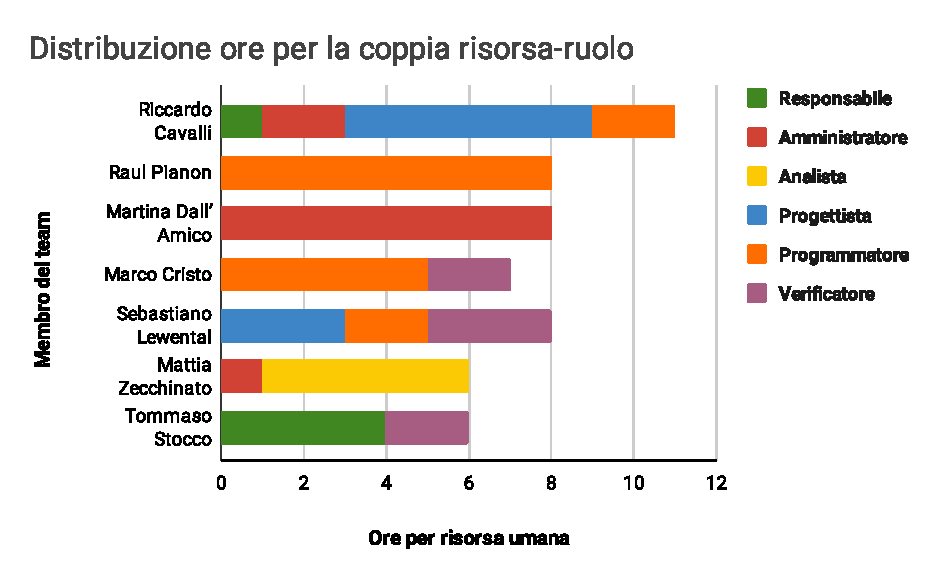
\includegraphics[width=0.90\textwidth]{assets/Consuntivo/Sprint-3/distribuzione_ore_risorsa_ruolo.pdf}
    \caption{Sprint 3 - Istogramma della distribuzione oraria per la coppia risorsa-ruolo}
  \end{figure}
  
  \begin{figure}[H]
    \centering
    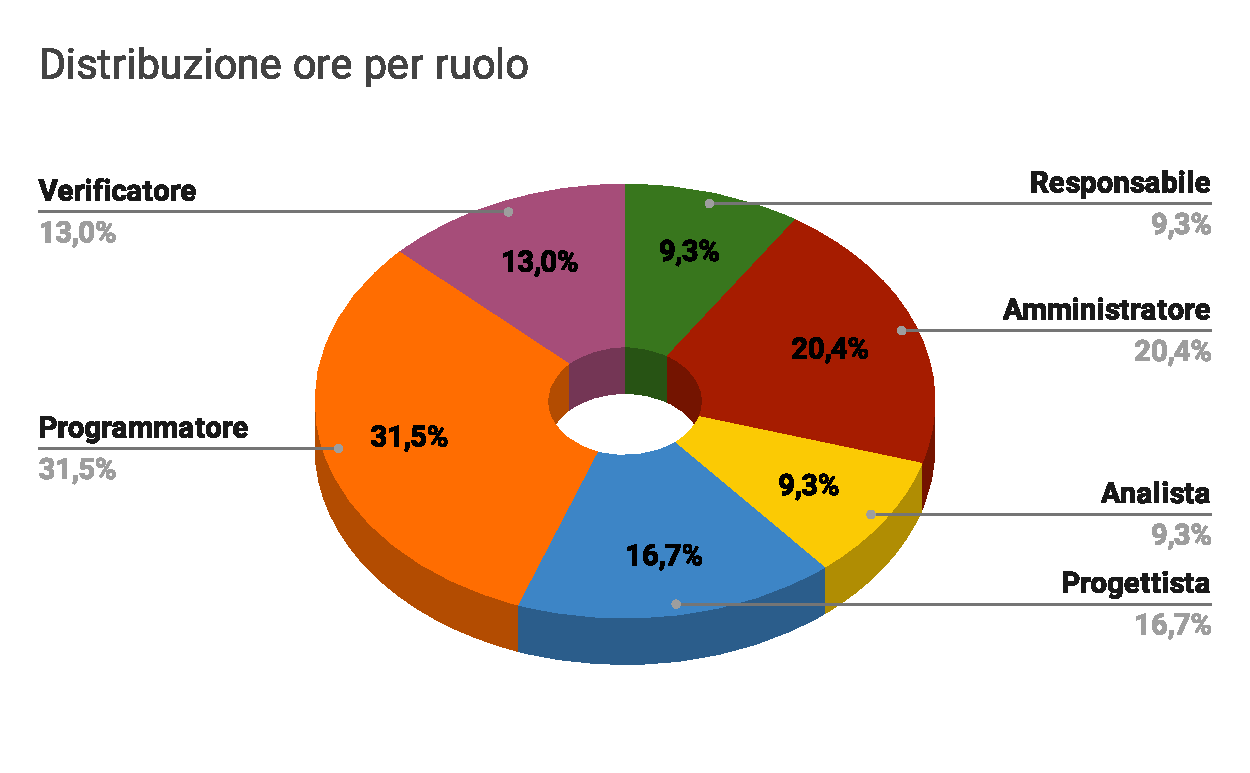
\includegraphics[width=0.90\textwidth]{assets/Consuntivo/Sprint-3/distribuzione_ore_ruolo.pdf}
    \caption{Sprint 3 - Areogramma della distribuzione oraria per ruolo}
  \end{figure}
  
  \begin{minipage}{\textwidth}
  Di seguito è riportato il consuntivo economico del terzo \glossario{sprint}:
  \begin{table}[H]
  \begin{adjustwidth}{-0.5cm}{-0.5cm}
    \centering
    \begin{tabular}{|P{2.9cm}|P{2.3cm}|P{2.5cm}|P{2.3cm}|>{\arraybackslash}P{2.5cm}|}
      \hline
      \multicolumn{5}{|c|}{\textbf{Consuntivo economico}} \\
      \hline
      \textbf{Ruolo} & \textbf{Ore per ruolo} & \textbf{Delta ore preventivo - consuntivo} & \textbf{Costo (in \texteuro)} & \textbf{Delta costo preventivo - consuntivo (in \texteuro)} \\
      \hline
      \Responsabile[U] & 5 & +1 & 150,00 & +30,00 \\ 
      \hline
      \Amministratore[U] & 11 & +1 & 220,00 & +20,00 \\ 
      \hline
      \Analista[U] & 5 & -1 & 125,00 & -25,00 \\ 
      \hline
      \Progettista[U] & 9 & -3 & 225,00 & -75,00 \\ 
      \hline
      \Programmatore[U] & 17 & -1 & 255,00 & -15,00 \\ 
      \hline
      \Verificatore[U] & 7 & 0 & 105,00 & 0,00 \\ 
      \hline
      \textbf{Totale} & \textbf{54} & -3 & \textbf{1.080,00} & -65,00 \\ 
      \hline
      \textbf{Restante} & 488 & / & 9.790,00 & / \\ 
      \hline
      \textbf{Sprint pregressi} & 95 & / & 2.150,00 & / \\ 
      \hline
    \end{tabular}
    \caption{Sprint 3 - Consuntivo economico}
  \end{adjustwidth}
  \end{table}
  \end{minipage}
  
  \begin{figure}[H]
    \centering
    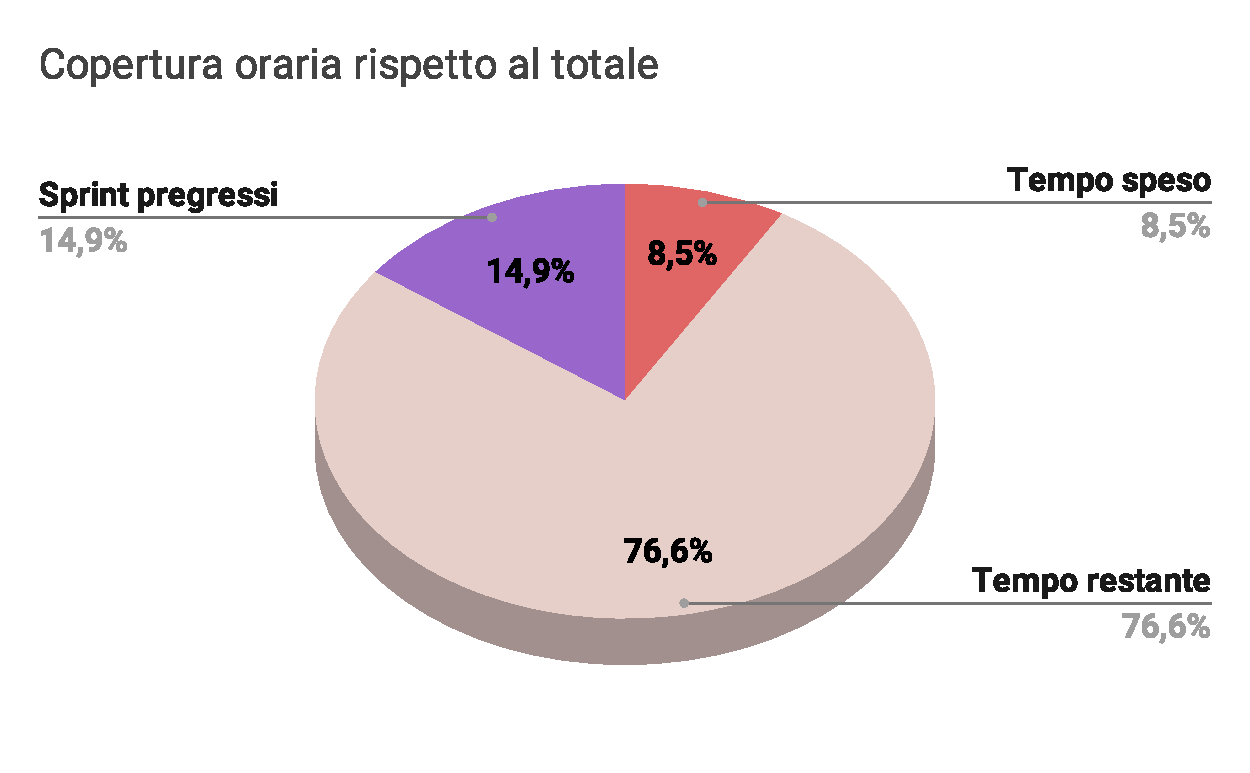
\includegraphics[width=0.90\textwidth]{assets/Consuntivo/Sprint-3/copertura_oraria.pdf}
    \caption{Sprint 3 - Areogramma del tempo speso (in ore) rispetto al totale}
  \end{figure}
  
  \begin{figure}[H]
    \centering
    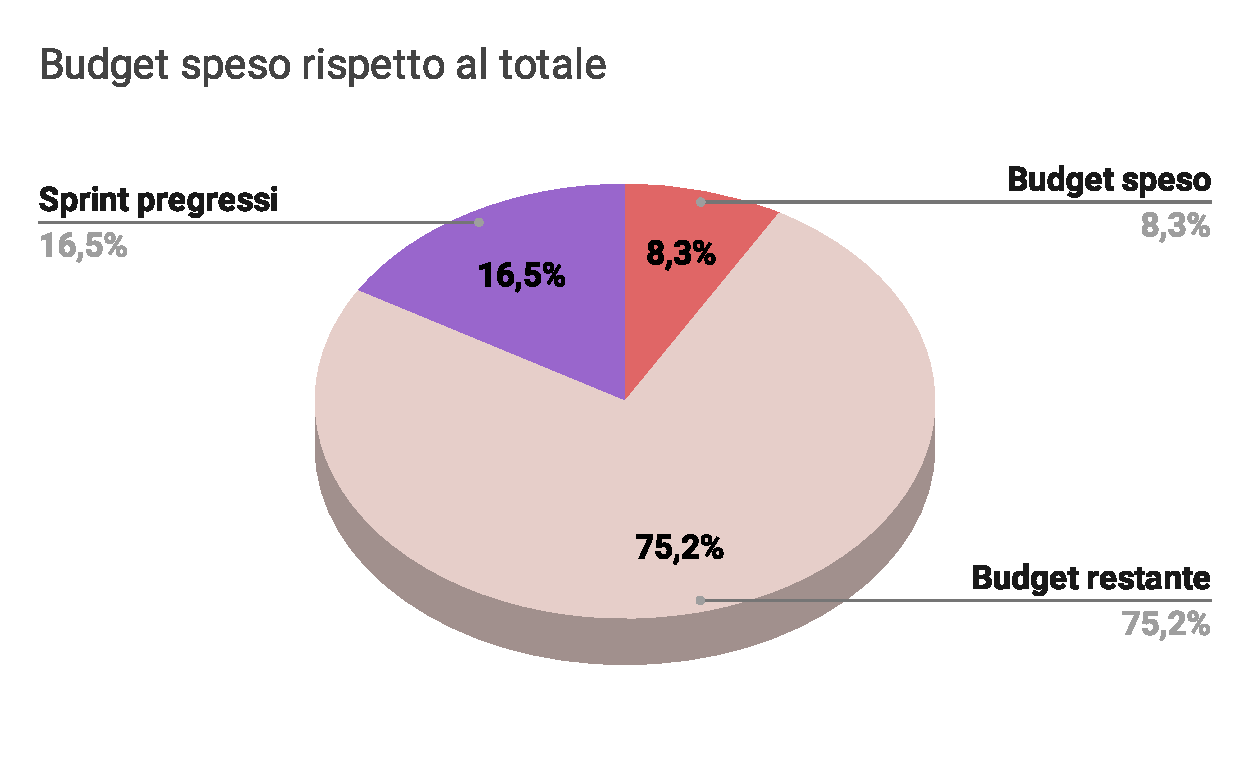
\includegraphics[width=0.90\textwidth]{assets/Consuntivo/Sprint-3/budget_speso.pdf}
    \caption{Sprint 3 - Areogramma del budget speso rispetto al totale}
  \end{figure}
  
  \begin{minipage}{\textwidth}
    Di seguito sono riportate le ore rimanenti per la coppia risorsa-ruolo:
    \begin{table}[H]
      \begin{tabularx}{\textwidth}{|c|*{6}{>{\centering}X|}c|}
        \hline
        \multicolumn{8}{|c|}{\textbf{Ore rimanenti per la coppia risorsa-ruolo}} \\
        \hline
        \textbf{Membro del team} & \textbf{Re} & \textbf{Am} & \textbf{An} & \textbf{Pt} & \textbf{Pr} & \textbf{Ve} & \textbf{Totale per persona} \\
        \hline
        Riccardo Cavalli & 0 & 0 & 9 & 17 & 20 & 20 & 66 \\ 
        \hline
        Raul Pianon & 2 & 8 & 9 & 23 & 14 & 12 & 68 \\ 
        \hline
        Martina Dall'Amico & 9 & 0 & 1 & 23 & 22 & 15 & 70 \\ 
        \hline
        Marco Cristo & 9 & 8 & 2 & 20 & 12 & 18 & 69 \\ 
        \hline
        Sebastiano Lewental & 9 & 8 & 2 & 14 & 20 & 17 & 70 \\ 
        \hline
        Mattia Zecchinato & 9 & 7 & 3 & 17 & 22 & 14 & 72 \\ 
        \hline
        Tommaso Stocco & 5 & 2 & 3 & 23 & 22 & 18 & 73 \\ 
        \hline
        \textbf{Totale ore per ruolo} & 43 & 33 & 29 & 137 & 132 & 114 & \textbf{488} \\ 
        \hline
      \end{tabularx}
      \caption{Sprint 3 - Ore rimanenti per la coppia risorsa-ruolo}
    \end{table}
  \end{minipage}

\subsubsection{Revisione delle attività}

Nell'arco del terzo \glossario{sprint}, il team ha svolto le seguenti attività:
\begin{itemize}
    \item Stesura verbali interni ed esterni;
    \item Push e pull dell'immagine \glossario{Docker} su \glossario{GitHub Container Registry};
    \item Aggiornamento delle \NdP\ con le modalità di integrazione Jira - Github;
    \item Riformulazione del dizionario dati (chiavi primarie, chiavi esterne e sinonimi);
    \item Creazione della prima bozza dell'interfaccia grafica;
    \item Studio del framework \glossario{Streamlit} e inizio sviluppo della web app;
    \item Definizione di un indice aggiuntivo per ricavare le informazioni delle tabelle pertinenti alla richiesta dell'utente;	
    \item Modifica struttura del PdP\ e approfondimento della sezione relativa al consuntivo;
    \item Selezione e descrizione delle metriche M1, M2, M3, M4;
    \item Scelta dei range di tolleranza per le metriche M1, M2, M3, M4;
    \item Benchmark iniziale dei modelli;
    \item Unificazione dei differenti metodi di estrazione del \glossario{dizionario dati} in un modulo unico;
    \item Stesura delle sezioni incomplete nel documento di \AdR;
    \item Espansione dei casi d'uso e rifinitura delle definizioni dei requisiti e delle fonti;
    \item Approfondimento del funzionamento di \glossario{txtai};
    \item Creazione di un dizionario dati in italiano per testare il modello sentence-BERTino di efederici;
    \item Prova di traduzione della richiesta utente;
    \item Costruzione della query SQL per la ricerca semantica;
    \item Aggiunta dei sinonimi delle tabelle e delle colonne nell'\glossario{indice};
    \item Miglioramento della ricerca semantica tramite la media pesata dei punteggi;
    \item Definizione di un workflow su GitHub Actions per il repository di sviluppo;
    \item Preventivo dello sprint 4;
    \item Elaborazione di una presentazione sul framework Streamlit;
    \item Configurazione di \glossario{Flask} e \glossario{Django} come framework back-end alternativi.
\end{itemize}

\subsubsection{Retrospettiva}

\par Di seguito sono riportati i risultati del questionario di valutazione dello \glossario{sprint}:
\begin{itemize}
  \item Organizzazione dello sprint - Valutazione: 8;
  \item Conduzione dei meeting interni - Valutazione: 8;
  \item Conduzione dei meeting esterni - Valutazione: 7,5;
  \item Impegno e partecipazione dei singoli membri - Valutazione: 8;
  \item La quasi totalità dei membri del team era a conoscenza delle proprie mansioni;
  \item La numerosità delle riunioni è adeguata, anche se il team preferirebbe organizzare più incontri informali tra membri che ricoprono ruoli affini;
  \item Le riunioni sono state organizzate quasi sempre con il giusto preavviso;
  \item Il rapporto ore spese/ore produttive è discreto, ma può essere ancora migliorato;
  \item La produttività generale deve essere incrementata;
  \item Alcuni membri del team ritengono sia necessario un maggior controllo sulle attività da parte del \Responsabile{}.
\end{itemize}

\vspace{0.5\baselineskip}
\par A seguire le \textbf{analisi a posteriori} del terzo \glossario{sprint}:
\begin{itemize}
  \item Nonostante quanto emerso dal consuntivo orario, dove l'assegnazione temporale per ruolo è risultata sbilanciata a favore dei ruoli più tecnici (\Analista{}, \Progettista{}, \Programmatore{}) rispetto a quelli amministrativi (\Amministratore{}, \Responsabile{}), il team ha ritenuto opportuno non allocare ulteriori risorse a questi ultimi per concentrare gli sforzi sullo sviluppo del PoC;
  \item In seguito alle considerazioni del team riguardo la necessità di una maggiore supervisione da parte del \Responsabile{}, quest'ultimo dovrà impegnarsi, a partire dalla prossima iterazione, a stabilire degli intervalli di tempo sufficientemente brevi alla fine dei quali verificare lo stato di avanzamento delle attività;
  \item La conduzione delle riunioni esterne ha evidenziato l'inesperienza del team nel rapporto con la \glossario{Proponente}, che assume a tutti gli effetti il ruolo di cliente, le cui conoscenze tecniche sono spesso asimmetriche rispetto a quelle dei fornitori. La discussione dei dettagli implementativi è un processo interno al gruppo e, pertanto, non deve coinvolgere il cliente. In futuro sarà quindi opportuno mantenere la discussione a un livello più alto, concentrandosi sul "cosa" piuttosto che sul "come";
  \item Malgrado le difficoltà nell'individuare gli standard per la gestione dei servizi IT, i membri con il ruolo di \Amministratore{} sono stati in grado di reperire sufficiente documentazione, seppur meno recente, per un'adeguata stesura delle metriche di qualità e la loro categorizzazione;
  \item Sebbene \glossario{Streamlit} abbia dei limiti dal punto di vista del design, il team ha deciso di investire un numero cospicuo di risorse nella progettazione dell'interfaccia grafica. In questo modo, qualora il gruppo dovesse scegliere di cambiare \glossario{framework}, la transizione risulterebbe meno gravosa.
\end{itemize}

\subsubsection{Aggiornamento pianificazione e preventivo}
\par Il team ha definito un piano d'azione per migliorare l'organizzazione e la produttività del prossimo \glossario{sprint}:
\begin{itemize}
  \item Ridurre la rendicontazione produttiva di ore spese per studi che non avanzano concretamente lo stato del progetto;
  \item Definire delle \glossario{metriche di qualità} da applicare nel corso dello sviluppo dell'applicativo e non in retrospettiva;
  \item Impostare dei test per valutare la correttezza del \glossario{prompt};
  \item Aumentare l'interazione tra analisti, progettisti e programmatori;
  \item Definire una vista dei log per analisi più puntuali dei risultati;
\end{itemize}

\paragraph*{Pianificazione futura:}
Data l'assenza di una suite di test automatici, il \glossario{benchmark} dei modelli di \glossario{sentence similarity} ha richiesto uno sforzo maggiore in termini di tempo e non ha prodotto risultati sufficientemente attendibili. Di conseguenza, il team ha aggiornato la pianificazione del prossimo \glossario{sprint}, fissando come task ad alta priorità la definizione dei test di unità. Mediante l'esecuzione automatica di una batteria di test, il gruppo ritiene di poter verificare con maggior rigore l'affidabilità dei modelli di AI scelti. Come definito nella \glossario{retrospettiva}, il team non ha ancora finalizzato la scelta delle tecnologie, in quanto lo sviluppo degli scenari critici verrà ultimato nel prossimo \glossario{sprint}. Pertanto, il gruppo ha stabilito di proseguire l'analisi di framework alternativi anche nel prossimo periodo, al termine del quale verrà presa una decisione definitiva. La \glossario{dockerizzazione} dell'ambiente di sviluppo, invece, è stata pianificata per lo \glossario{sprint} 5. Le dipendenze del progetto verranno infatti delineate nell'arco della prossima iterazione.
\par Per quanto riguarda le metriche di qualità, il team ha fissato i seguenti obiettivi:
\begin{itemize}
  \item Individuazione delle metriche più significative;
  \item Identificazione di strumenti per automatizzare il calcolo delle metriche.
\end{itemize}
\par Dopo aver preso in considerazione un ampio insieme di indicatori, il gruppo ritiene infatti necessario operare una scrematura delle metriche individuate.

\paragraph*{Preventivo "a finire" (\sezione{sec:stima_temporale}):}
Il consuntivo del terzo \glossario{sprint} ha evidenziato una discrepanza di tre ore produttive rispetto a quanto preventivato. Questo perché la maggior parte del tempo è stata impiegata nello studio e nella valutazione delle tecnologie per il \glossario{PoC}. Nonostante i programmatori abbiano iniziato lo sviluppo del prototipo con \glossario{Streamlit}, il team ha ritenuto opportuno esaminare \glossario{framework} alternativi come \glossario{Django}, \glossario{Vue.js} e \glossario{Next.js}. Inoltre, l’uso delle funzionalità avanzate di \glossario{txtai} e la progettazione della bozza dell’interfaccia grafica hanno richiesto una fase di studio non indifferente. Per tale motivo, il gruppo ha deciso di rivedere il calendario di massima del progetto. Nel prossimo sprint, infatti, il team si focalizzerà sullo sviluppo dei \glossario{casi d’uso} all’interno dell’applicazione. Qualora la risposta di \glossario{Streamlit} dovesse risultare negativa (in termini di flessibilità, prestazioni e personalizzazione), il gruppo dovrebbe optare per due nuovi framework (back-end e front-end). Dunque, il team ha ridefinito la finestra temporale per la revisione \glossario{RTB} come segue:
\begin{itemize}
  \item Data di inizio: 2024-06-03;
  \item Scadenza: 2024-06-14.
\end{itemize}

\paragraph*{Gestione dei rischi (\sezione{sec:analisi_rischi}):}
\par Nel corso del terzo \glossario{sprint}, il team ha riscontrato l'affioramento di due rischi inattesi:
\begin{itemize}
  \item \textbf{RP1 - Questioni personali}: nonostante il largo anticipo della comunicazione, l'impossibilità di uno dei membri del team di svolgere i propri incarichi, ha comportato la ridistribuzione di questi ultimi tra i restanti membri dai ruoli affini. Questa forma di mitigazione ha avuto un successo parziale: lo sviluppo dell'\AdR\, seppur non interrotto, ha subito rallentamenti. Di conseguenza, il team ha ritenuto opportuno l'ampiamento della \sezione{sec:analisi_rischi} con una sottosezione relativa ai rischi di natura personale, rifinendo l'approccio adottato al netto dei rallentamenti come misura di mitigazione finale;
  \item \textbf{RT3 - Malfunzionamenti software}: la configurazione di \glossario{Docker} e dell'ambiente di sviluppo ha causato malfunzionamenti software. Tuttavia, l'organizzazione tempestiva di incontri su Discord tra i membri interessati e i componenti con più esperienza ha risolto tali problematiche.
\end{itemize}

\par Inoltre, alcune contromisure si sono rivelate insufficienti a mitigare i rischi emersi:
\begin{itemize}
  \item \textbf{RO6 - Risorse disponibili ma non impiegate}: con una pianificazione più accorta, alcuni membri del team, impiegati in attività di studio e test ancora premature, avrebbero potuto supportare il lavoro dei programmatori.
\end{itemize}

\vspace{0.5\baselineskip}
\par Di seguito sono elencati i rischi gestiti con successo:
\begin{itemize}
  \item \textbf{RO2 - Collaborazione}: durante il terzo \glossario{sprint}, il team ha ritenuto opportuno raccogliere, confrontare e infine integrare le opinioni (talvolta discordanti) di ciascun membro riguardo le regole interne, al fine di garantire una collaborazione proficua e continua tra i membri;
  \item \textbf{RO4 - Rotazione dei ruoli}: durante i primi \glossario{sprint}, diversi membri del gruppo hanno mantenuto le stesse mansioni per l'intera durata dell'iterazione, non riuscendo ad approfondire le proprie conoscenze al di fuori del ruolo assegnato. Questo ha provocato incertezze durante la rotazione dei ruoli da uno sprint all'altro. Le riunioni frequenti e il sostegno reciproco durante la transizione dei ruoli sono stati fondamentali per compensare la mancanza di esperienza;
  \item \textbf{RT1 - Scarso know-how tecnologico}: i nuovi programmatori sono stati affiancati dai membri del team che avevano già ricoperto quel ruolo, riducendo così la curva di apprendimento di \glossario{txtai}.
\end{itemize}
